\chapter{Project Scope and Planning}

\section{Introduction}
This chapter is dedicated to a comprehensive analysis of system requirements, encompassing both functional and non-functional attributes necessary to meet our user needs. Subsequently, a suitable project management methodology will be selected to finally outline a project plan, including task delineation and associated deadlines.

\section{Project Requirements}
In this section, we outline the comprehensive requirements for the project, essential for breaking down the project goals into tasks and guiding development efforts.\newline
First, we start by outlining the main actors involved in the system's functioning.
\subsection{Actors Identification}
An actor is an abstract representation of an entity which interacts with the system being conceived. This element can be a user, a group of users, or an external system, which trigger the system's processes.\newline
The actors are categorized as follows:
\begin{itemize}
    \item \textbf{Regular User:} This role represents an employee who has access to use the application, which provides them with answers to their questions based on content stored in vector databases.
    \item \textbf{Database Manager:} A DB manager is a regular user that has access to authentication keys for a database. In addition to the regular features which a normal user has access to, this role allows them to access and index new content into a shared database.
    \item \textbf{Administrator:} The role of the application administrator is to manage the default configuration and parameters of the application.
\end{itemize}
\subsection{Functional Requirements}
After identifying the different actors of the system, we will describe the features which will be integrated in the system and assign them to these roles.
\subsubsection{Regular User}
\begin{itemize}
    \item \textbf{Response source choice:} The system should allow users to pick the vector databases from which information relevant to their queries will be retrieved.
    \item \textbf{Data augmentation:} The system should provide external knowledge feteching methods to allow the ingestion of related information from real-time sources.
    \item \textbf{Translation:} The system should enforce cross language capabilities for accurate and consistent behavior in a multilingual context.
    \item \textbf{Model Selection:} The system must integrate different Generative AI models from which a user can select options relative to the API they have access to.
    \item \textbf{Answers:} The system must be able to process user queries, retrieving relevant information from the selected databases and generating answers based on users choices, and then prioritize the more informative responses.
    \item \textbf{Feedback options:} The system should allow users to give their feedback for each response result, and use this feedback when ranking further answers.
\end{itemize}
\subsubsection{Database Manager}
\begin{itemize}
    \item \textbf{Database authentication:} The system should allow users to gain database management access with a DB name and passphrase.
    \item \textbf{Database management:} The system must allow DB managers to access the DB content and index new information into it.
\end{itemize}
\subsubsection{Application Administrator}
\begin{itemize}
    \item \textbf{Configuration management:} The system should provide options for the Administrator to change the default configuration: API keys, initial databases with names and passphrases for different teams, and changing the directory for storing application data and cache.
\end{itemize}
\subsection{Non-function Requirements}
In addition to the functionalities that the application must provide for its users, there are other characteristics and attributes which the project must respect and pursue. These constraints do not describe the services made available for the end user, but rather focus on their quality and performance.
\begin{itemize}
    \item \textbf{Performance:} The time it takes for Loading, using and navigating pages of the app should be minimal, even in the case of multiple simultaneous connections.
    \item \textbf{Conviviality and Usability:} The interfaces should be intuitive and accessible.
    \item \textbf{Maintainability:} The source code should be organized to allow the improvement and evolution of the project.
\end{itemize}

\section{Project Management}
Upon establishing the project's requirements and functionalities, it is now time to plan out expected tasks into an organized timetable. This section of the chapter addresses that. It is composed of two parts, one explaining the suitability of the employed methodology throughout the project, and another detailing the tasks to be undertaken.
\subsection{Methodology}
Given the nature of this project, the Scrum methodology was selected for the implementation of the system. This iterative approach allowed for the continuous development and refinement of tasks (Sprints) throughout this internship by allowing users' interference and feedback during the development process. This flexibility was particularly valuable in this end-of-studies project where the final requirements kept evolving.
\begin{figure}[H]
    \centering
    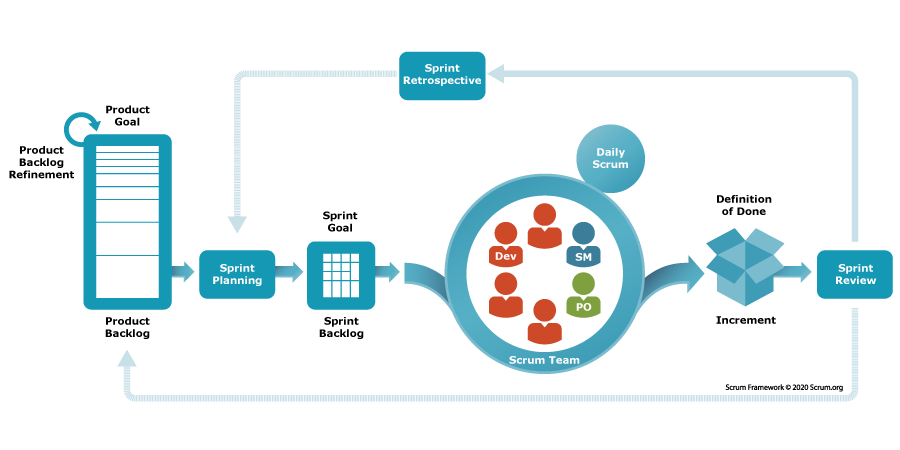
\includegraphics[width=\linewidth]{./figures/scrum-framework-9.29.23.png}
    \caption{Scrum framework \href{https://www.scrum.org/resources/what-scrum-module}{[What is Scrum (scrum.org)]}}.
\end{figure}
This methodology defines the steps to implement a project as follows :
\begin{enumerate}
    \item Project Planning : Defining the project's overall objectives and values to be gained by users. And on a smaller scale, the specific Sprint objectives.
    \item Product Backlog : Identifying and re-prioritizing the customer's requirements into an organized list of Sprints.
    \item Sprints : Identifying and organizing tasks into a list of Sprints
    \item Scrum Meetings : Daily short meetings to discuss progress and challenges to complete a Sprint's tasks.
    \item Increment development : Iteratively complete Sprint cycles (planning, design, coding, testing and review) to complete increments.
    \item Sprint Review : Review of the completed work with the entreprise supervisor
    \item Sprint Retrospective : Discussing what went good and what went bad during the Sprint to gain better insight on what can be improved in the future.
\end{enumerate}
The following section demonstrates the influence of this agile methodology, by showcasing a planned timetable in compliance with the iterative approach of the Scrum methodology.
\subsection{Planning}
\begin{figure}[H]
    \centering
    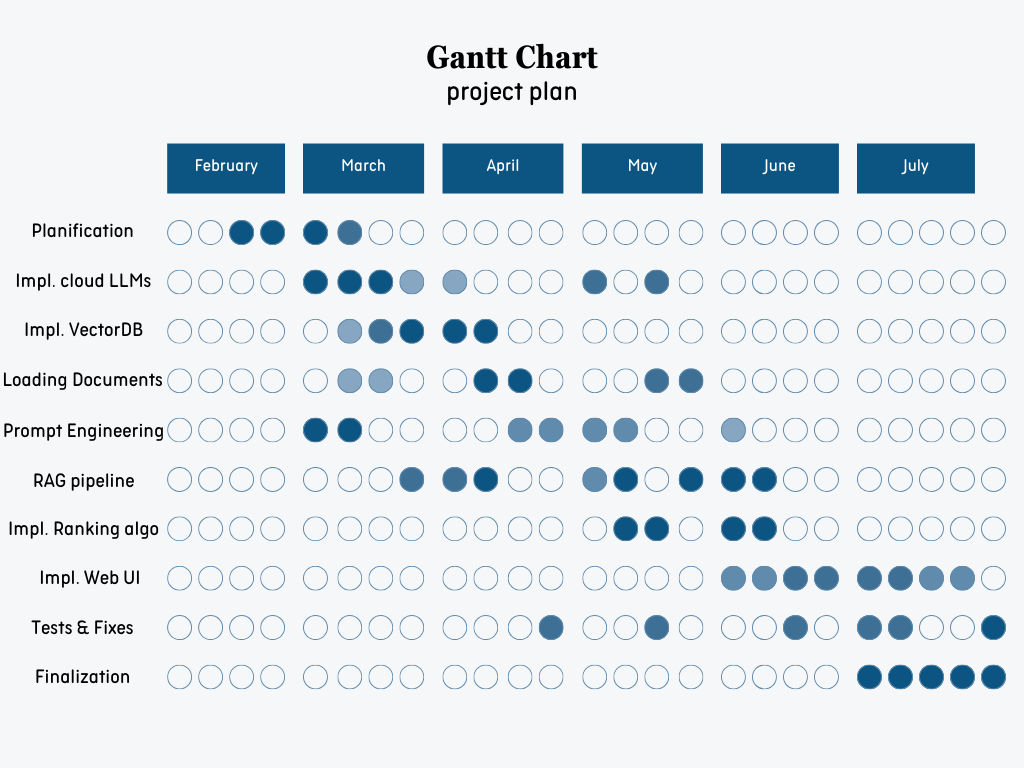
\includegraphics[width=\linewidth]{./figures/gantt-chart-1.png}
    \caption{The planned Gantt Chart}
    \begin{flushleft}
        \par This Gantt Chart illustrates the timetable of planned tasks and how they were split over smaller chunks to accomplish them and iterate the development process over different segments. This method allowed to accomplish Increments, which represent tangible steps towards the final project implementation: The first iteration (second week of March) was planned to implement Large Language Models standalone answering functionality (without RAG or a vector store), combining cloud-based LLMs with prompt engineering techniques. The next iteration focused on initiating the RAG pipeline by implementing a vector store index with static content, modifying Prompts to control the LLMs' factual grounding, after which some testing and further development was conducted to tailor to the different LLMs and make the vector store more dynamic by implementing data augmentation methods. After these two iterations which were completed by the start of May, further enhancement was undertaken to customize the indexing methods to tailor to different teams and the retrieval phase to minimize dissimilar results, in addition to supplying more data augmentation knowledge sources through APIs and the exploration of how a ranking algorithm could be implemented. The final iteration focused on integrating all the functionalities into a web interface, implementing a user feedback option and enhance answer ranking and validating the results with the corporate supervisor.
    \end{flushleft}
\end{figure}

\section{Conclusion}
This chapter, along with the previous one, clarified the project's roadmap and helped breaking down the problem statement into a list of tasks to be implemented. These tasks are now explained in more detail in the following chapter, which discusses the implementation phase of this project.